% % document's head

\begin{center}
    \LARGE \textsc{Название}
\end{center}

\hrule

\phantom{42}

\begin{flushright}
    \begin{tabular}{rr}
    % written by:
        % \textbf{Источник}: 
        % & \href{__ссылка__}{__название__} \\
        % & \\
        % \textbf{Лектор}: 
        % & _ФИО_ \\
        % & \\
        \textbf{Авторы заметок}: 
        & Хоружий Кирилл \\
        % & Примак Евгений \\
        & \\
    % date:
        \textbf{От}: &
        \textit{\today}\\
    \end{tabular}
\end{flushright}

\thispagestyle{empty}
\tableofcontents
\newpage



% % Lorem ipsum dolor sit amet, consectetur adipisicing elit, sed do eiusmod
% tempor incididunt ut labore et dolore magna aliqua. Ut enim ad minim veniam,
% quis nostrud exercitation ullamco laboris nisi ut aliquip ex ea commodo
% consequat. Duis aute irure dolor in reprehenderit in voluptate velit esse
% cillum dolore eu fugiat nulla pariatur. Excepteur sint occaecat cupidatat non
% proident, sunt in culpa qui officia deserunt mollit anim id est laborum.
% \begin{equation*}
% 	\ket{\psi} = \alpha_1 \raisebox{-6.3mm}{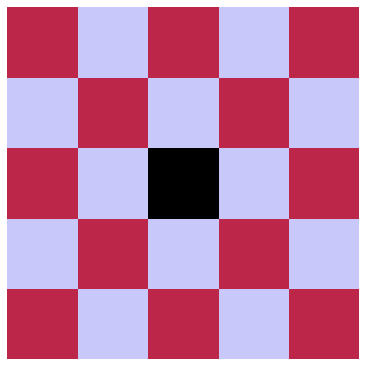
\includegraphics[width=0.08\textwidth]{s1.pdf}} + 
% 	\alpha_2 \raisebox{-6.3mm}{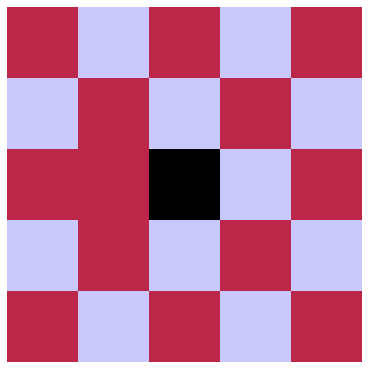
\includegraphics[width=0.08\textwidth]{s2.pdf}} + 
% 	\alpha_3 \raisebox{-6.3mm}{
\includegraphics[width=0.08\textwidth]{s3.pdf}} + \ldots
% \end{equation*}

% \begin{equation*}
% 	\hat{H} = J \sum_{\langle i,j\rangle} \hat{S}_i \hat{S}_j - t \sum_{\langle i,j\rangle} \hat{c}_i\D \hat{c}_j
% \end{equation*}

% \begin{equation*}
% 	f(z) = \left\{\begin{aligned}
% 	    &1 - {\tilde{N}^0_{\text{pred}> z}}/{\tilde{N}^1_{\text{pred}< z}}, &z \geq \text{treshold} \\
% 	    &{\tilde{N}^1_{\text{pred}< z}}/{\tilde{N}^0_{\text{pred}> z}}-1, &z < \text{treshold} \\
% 	\end{aligned}\right.
% \end{equation*}


% \begin{equation*}
% 	f(z) = \tilde{N}^1_{\text{pred}< z}
% \end{equation*}


%  \begin{equation*}
%  	\hat{H} = - \sum_{\langle i,j\rangle} \hat{c}_i\D \hat{c}_j
%  \end{equation*}

%  \begin{equation*}
%  	g_2(r) = \langle \hat{c}_{\vc{j}}\D \hat{c}_{\vc{j}+\vc{r}}\D \hat{c}_{\vc{j}+\vc{r}}\hat{c}_{\vc{j}}\rangle_{\vc{j}}
%  \end{equation*}

%  \begin{equation*}
%  	\sub{\hat{H}}{FH} = - t \sum_{\langle i,j\rangle, \sigma} \hat{c}_{i \sigma}\D \hat{c}_{j \sigma} + U \sum_j \hat{n}_{j \uparrow} \hat{n}_{j \downarrow} + \sum_{j, \sigma} (V_j - \mu)\hat{n}_{j, \sigma}
%  \end{equation*}

%  \begin{equation*}
%  	{\hat{H}}_{tJ} = - t \sum_{\langle i,j\rangle, \sigma} \hat{c}_{i \sigma}\D \hat{c}_{j \sigma} + J \sum_{\langle i,j\rangle}\left(
%  		\hat{S}_i \hat{S}_j - \tfrac{1}{4} n_i n_j
%  	\right) + O(t^3 / U^2)
%  \end{equation*}

%  \begin{equation*}
%  	\langle \hat{O}\rangle(T) = \tfrac{1}{Z}\sum_j e^{- E_j / T} \bk{\psi_j}[\hat{O}]{\psi_j}
%  \end{equation*}

% \begin{equation*}
% {\hat{H}}_{tJ} = - t \sum_{\langle i,j\rangle, \sigma} \hat{c}_{i \sigma}\D \hat{c}_{j \sigma} + J \sum_{\langle i,j\rangle}
% 	\hat{S}_i \hat{S}_j
% \end{equation*}

% Stern-Gerlach: $F = \mu_z  \cdot \tfrac{\partial B}{\partial z} $



% \begin{equation*}
% 	\begin{pmatrix}
% 		\text{cost}_1 \\ \ldots \\ \text{cost}_n
% 	\end{pmatrix} \to \begin{pmatrix}
% 		w_1 \cdot \text{cost}_1 \\ \ldots \\ w_n \cdot  \text{cost}_n
% 	\end{pmatrix} 
% \end{equation*}



% \setcounter{section}{2}
% 

We could consider
\begin{equation*}
	\ket{\alpha_1,\ldots,\alpha_N} = \frac{1}{\sqrt{N!}} \sum_{P} \zeta^{\sigma(P)} 
	\ket{\alpha_{P(1)}} \otimes \ldots \otimes \ket{\alpha_{P(N)}},
\end{equation*}
where $\zeta= \pm 1$ for bosons and fermions respectively. We define creation operator via
\begin{equation*}
	a_{\beta}\D \ket{\alpha_1,\ldots,\alpha_N} \overset{\mathrm{def}}{=} \ket{\beta,\alpha_1,\ldots,\alpha_N}.
\end{equation*}
\begin{enumerate}
	\item Adjoint $a_\beta$ could be expressed as
	\begin{align*}
		a_\beta\D &= \sum_{\{\theta\}} \kb{\beta, \theta_1, \ldots, \theta_M}{\theta_1, \ldots, \theta_{M}}, \\
		a_\beta &= \sum_{\{\theta\}} \kb{\theta_1, \ldots, \theta_M}{\beta, \theta_1, \ldots, \theta_{M}}.
	\end{align*}
	Than it could be shown that
	\begin{equation*}
		a_\beta \ket{\alpha_1,\ldots,\alpha_N} = \sum_k C_k \ket{\alpha_1,\ldots,\cancel{\alpha_k},\ldots,\alpha_N},
	\end{equation*}
	with 
	\begin{align*}
		C_k = \bk{\beta,\alpha_1,\ldots,\cancel{\alpha_k},\ldots,\alpha_N}{\alpha_1,\ldots,\alpha_N} 
		= \frac{1}{\sqrt{N!}}\sum_{P} \bra{\alpha_{P(1)}} \otimes \ldots \otimes \bra{\beta}_{P(k)} \otimes \ldots \otimes \bra{\alpha_{P(N)}} \alpha_1,\ldots,\alpha_N \big\rangle,
	\end{align*}
	where we could <<move>> $\bra{\beta}$  to the start, by $P(k)-1$ transpositions, and due to $N!$ equal permutations we could neglect $\frac{1}{N!}$  coming to
	\begin{equation*}
		C_k = \zeta^{k-1} \bk{\beta}{\alpha_k}.
	\end{equation*}
	\item We also could find, that $a_\beta$ and $a_\beta\D$ fuldill the (anti)-commutation relations 
	\begin{align*}
		a_\beta\D a_\alpha \ket{\theta_1,\ldots,\theta_N} &= a_\beta\D \sum_{k=1}^{N} \zeta^{k-1} \bk{\alpha}{\theta_k} \ket{\theta_1,\ldots,\cancel{\theta_k},\ldots,\theta_N} = \sum_{k=1}^{N} \zeta^{k-1} \bk{\alpha}{\theta_k} \ket{\beta,\theta_1,\ldots,\cancel{\theta_k},\ldots,\theta_N}, \\
		a_\alpha a_\beta\D \ket{\theta_1,\ldots,\theta_N} &= a_\alpha \ket{\beta,\theta_1,\ldots,\theta_N} = \sum_{k=1}^{N} \zeta^{k} \bk{\alpha}{\theta_k} \ket{\beta,\theta_1,\ldots,\cancel{\theta_k},\ldots,\theta_N} + \bk{\alpha}{\beta} \ket{\theta_1,\ldots,\theta_N},
	\end{align*}
	so for bosons $\zeta=1$ we have
	\begin{equation*}
		[a_\alpha, a_\beta\D] \overset{\mathrm{def}}{=} a_\alpha a_\beta\D - a_\beta\D a_\alpha = \bk{\alpha}{\beta} = \delta_{\alpha,\beta},
	\end{equation*}
	and in the same way for fermions $\zeta=-1$ and
	\begin{equation*}
		\{a_\alpha, a_\beta\D\} \overset{\mathrm{def}}{=} a_\alpha a_\beta\D + a_\beta\D a_\alpha = \bk{\alpha}{\beta} = \delta_{\alpha,\beta}.
	\end{equation*}
	\item For density operator 
	\begin{equation*}
		\hat{\rho}(x) = \sum_{j=1}^{N} \delta(x-\hat{x}_j),
	\end{equation*}
	we could find second quantized form
	\begin{equation*}
		\hat{\rho}(x) = \sum_{\alpha \beta} \bk{\alpha}[\delta(x-\hat{x})]{\beta} \hat{a}_\alpha\D \hat{a}_\beta = \sum_{\alpha \beta} \int
		\bk{\alpha}{x'} \bk{x'}{\beta} \delta(x-x') \d x' \hat{a}_\alpha\D \hat{a}_\beta = \sum_{\alpha \beta} \bk{\alpha}{x} \bk{x}{\beta} \hat{a}_\alpha\D \hat{a}_\beta,
	\end{equation*}
	what could be reduced to the $\hat{a}_x\D \hat{a}_x$ form if $\ket{\alpha}$ and $\ket{\beta}$ corresponds to the coordinates.
\end{enumerate}

\begin{equation*}
	\vc{\alpha} + \tilde{\hat{\vc{\beta}}} + 
\end{equation*}
% \newpage
% 

We could rewrite classical 1D Ising chain partitin function as
\begin{equation*}
	\sub{\mathcal{Z}}{c} = T_{s_1,s_2} \ldots T_{s_{N-1},s_{N}} T_{s_N, s_1} = \tr\left(T^N\right),
\end{equation*}
with transfer matrix
\begin{equation*}
	T = T^a T^b = \left(
\begin{array}{cc}
 e^{h_\text{c}+K_\text{c}} & e^{h_\text{c}-K_\text{c}} \\
 e^{-h_\text{c}-K_\text{c}} & e^{K_\text{c}-h_\text{c}} \\
\end{array}
\right),
	\hspace{10mm}
	T^a = \begin{pmatrix}
	    e^{\Hc} & 0 \\
	    0 & e^{-\Hc} \\
	\end{pmatrix} 
	,\ \ \ 
	T^{b} = \begin{pmatrix}
	    e^{\Kc } & e^{-\Kc } \\
	    e^{-\Kc } & e^{\Kc } \\
	\end{pmatrix}.
\end{equation*}
There are different ways to define $T$,because important just eigenvalues
\begin{equation*}
	\lambda_{1,2} = \frac{1}{2} e^{-h_{\text{c}}-K_{\text{c}}} \left(e^{2 \left(h_{\text{c}}+K_{\text{c}}\right)}+e^{2 K_{\text{c}}} \pm \sqrt{ e^{4 K_{\text{c}}} \left(e^{2 h_{\text{c}}}-1\right)^2 +4 e^{2 h_{\text{c}}}}\right).
\end{equation*}
For a quantum system the partitin function 
\begin{equation*}
	\sub{\mathcal{Z}}{q} = \tr e^{-\beta H},
\end{equation*}
and we want to achieve
\begin{equation*}
	\sub{\mathcal{Z}}{q} = \sub{\mathcal{Z}}{c} = \tr\left(
		e^{-\frac{\beta}{N}H_1} e^{-\frac{\beta}{N}H_2}
	\right)^N,
	\hspace{10 mm} 
	e^{- \frac{\beta}{N} H_1} = T^a,
	\hspace{5 mm} 
	e^{- \frac{\beta}{N} H_2} = T^b.
\end{equation*}
Using formulas to the Pauli matrix exponents, we could find
\begin{equation*}
	H_1 = \frac{N}{-\beta} \alpha_3 \sigma_z,
	\hspace{10 mm} 
	H_2 = \frac{N}{-\beta} (\alpha_0 \1 - \alpha_1 \sigma_x),
\end{equation*}
with $\alpha_0 = \ln \sh(2 \Kc) + \ln 2$, $\alpha_1 = \ln \th \Kc$ and $\alpha_3 = \Hc$. I think it is possible to find other $H_1$ and $H_2$, my choice was ruled by separating $\Kc$ and $\Hc$ dependences.


% 
\phantom{42}

\vfill

\phantom{42} \hfill \textbf{\textit{\today, \ Khoruzhii Kirill}}



% \newpage
% \setcounter{section}{3}
% \setcounter{subsection}{0}
% \subsection{The Transverse Field Ising Model}
% 

Consider the Hamiltonian of the Transverse Field Ising Model (TFIM)
\begin{equation*}
	\hat{H} = - J \sum_{\langle i,j\rangle}
		\hat{\sigma}^x_i \hat{\sigma}^x_j
	- h \sum_j \hat{\sigma}_j^z
\end{equation*}
where $J,h>0$ with PBC $\hat{\sigma}_L^x \hat{\sigma}_{L+1}^x = \hat{\sigma}_{L}^x \hat{\sigma}_1^x$.


\begin{enumerate}
	\item We could try to map spins to bosonic operators
\begin{equation*}
	\left\{\begin{aligned}
		\hat{\sigma}_j^x &= \hat{b}_j+\hat{b}_j\D \\
		\hat{\sigma}_j^y &= i(\hat{b}_j\D-\hat{b}_j) \\
		\hat{\sigma}_j^z &= 1 - 2 \hat{b}_j\D \hat{b}_j
	\end{aligned}\right.
	\hspace{5 mm} \Leftrightarrow \hspace{5 mm} 
	\left\{\begin{aligned}
	    \hat{b}_j &= \hat{\sigma}_j^+ = \tfrac{1}{2}\hat{\sigma}_j^x + \tfrac{i}{2}\hat{\sigma}_j^y \\
	    \hat{b}_j\D &= \hat{\sigma}_j^- = \tfrac{1}{2}\hat{\sigma}_j^x - \tfrac{i}{2}\hat{\sigma}_j^y 
	\end{aligned}\right.
\end{equation*}

\begin{enumerate}[label=(\alph*)]
    \item  Bosons as define above are <<hard-core bosons>>. We know that
\begin{equation*}
	\left[\hat{\sigma}_i,\hat{\sigma}_j\right] = 0 \ \text{with} \  i \neq j,
	\hspace{5 mm} 
	\left[\hat{\sigma}^a,\hat{\sigma}^b\right] = 2 i \varepsilon_{abc} \hat{\sigma}^c,
	\hspace{5 mm} 
	\left\{\hat{\sigma}^a,\hat{\sigma}^b\right\} = 2 \delta_{ab} .
\end{equation*}
So bosons commute at different sites, but 
\begin{equation*}
	\{\hat{b}_j,\hat{b}_j\D\} = \tfrac{1}{2} \hat{\sigma}^x_i \hat{\sigma}^x_i +  \tfrac{1}{2} \hat{\sigma}^y_j \hat{\sigma}^y_j  = \1,
	\hspace{10 mm} 
	\hat{b}_j\D \hat{b}_j\D = \tfrac{1}{4}\hat{\sigma}_j^x \hat{\sigma}_j^x-\tfrac{1}{4}\hat{\sigma}_j^y \hat{\sigma}_j^y + \tfrac{1}{4}\{\hat{\sigma}_j^x, \hat{\sigma}_j^y\} = 0,
\end{equation*}
thus at most one boson is allowed on each site.

    \item  In 1D it's useful to modify bosons to spinless fermions by \textit{Jordan Wigner transformation}
\begin{equation*}
	\hat{b}_j = \hat{K}_j \hat{c}_j = \hat{c}_j \hat{K}_j,
	\hspace{10 mm} 
	\hat{K}_j = \prod_{i=1}^{j-1} (1-2 \hat{n}_i) = \pm 1, 
\end{equation*}
where non-local string operator $\hat{K}_j$ corresponds just to a sign and $\hat{K}_j = \hat{K}_j\D = \hat{K}_j^{-1}$. So if $\hat{c}$ are fermions then $\hat{b}$ satisfies the commutation and anticommutation relations 
\begin{equation}
\renewcommand{\arraystretch}{1.4}
	\begin{tabular}{ccc}
	$[\hat{b}_i, \hat{b}_j] = 0,$ & $[\hat{b}_i, \hat{b}_j\D] = 0,$ & $[\hat{b}_i\D, \hat{b}_j\D] = 0,$ \\
	$\{\hat{b}_j, \hat{b}_j\} = 0,$ & $\{\hat{b}_j, \hat{b}_j\D\} = 0,$ & $\{\hat{b}_j\D, \hat{b}_j\D\} = 0.$
	\end{tabular}
	\label{P12}
\end{equation}
Second row could be proven using
\begin{equation*}
	\hat{b}\D_j \hat{b}_j = \hat{c}_j\D \hat{K}_j\D \hat{K}_j \hat{c}_j = \hat{c}_j\D \hat{c}_j,
	\hspace{5 mm} 
	\hat{b}\D_j \hat{b}_j\D = \hat{c}_j\D \hat{K}_j\D \hat{K}_j\D \hat{c}_j\D = \hat{c}_j\D \hat{c}_j\D,
	\hspace{5 mm} 
	\hat{b}_j \hat{b}_j = \hat{c}_j \hat{K}_j \hat{K}_j \hat{c}_j = \hat{c}_j \hat{c}_j.
\end{equation*}
And without loss of generality for $j>i$
\begin{equation*}
	\hat{b}_i \hat{b}_j\D = \hat{c}_i \hat{K}_{i,j} \hat{c}_j\D,
	\hspace{5 mm} 
	\hat{b}_j\D \hat{b}_i = \hat{c}_j\D \hat{K}_{i,j} \hat{c}_i \overset{1}{=}  -\hat{K}_{i,j} \hat{c}_i   \hat{c}_j\D \overset{2}{=} \hat{c}_i \hat{K}_{i,j} \hat{c}_j\D,
	\hspace{0.5cm} \Rightarrow \hspace{0.5cm}
	[\hat{b}_i, \hat{b}_j\D] = 0,
\end{equation*}
with $\hat{K}_{i,j} = \prod_{k=i}^{j}(1-2\hat{n}_k)$. It was used in $\overset{1}{=}$ that 
$\{\hat{c}_i, \hat{c}_j\D\}=0$ and in $\overset{2}{=}$ that $\hat{c}_i$ changes parity for $\hat{K}_{i,j}$. The operators conjugation does not change the calculations, so we have proved \eqref{P12}. We need carefully work with PBS
\begin{equation*}
	\hat{b}_L\D \hat{b}_{1} = \hat{K}_L \hat{c}_L\D \hat{c}_1 \overset{3}{=}  -\left( \textstyle \prod_{i=1}^{L} (1-2 \hat{c}_i\D \hat{c}_i)\right) \hat{c}_L\D \hat{c}_1 = - (-1)^{\hat{N}}  \hat{c}_L\D \hat{c}_1,
	\hspace{10 mm} 
	\hat{N} = \sum_{j=1}^{L} \hat{c}_j\D \hat{c}_j,
\end{equation*}
where we used in $\overset{3}{=}$ that $j$-site occupied and we could complete to $- (-1)^{\hat{N}} $.


    \item  Summarising, spins are mapped into fermions using
\begin{equation*}
	\left.\begin{aligned}
	    \hat{\sigma}_x &= \hat{K}_j(\hat{c}_j\D + \hat{c}_j) ,\\
	    \hat{\sigma}_y &= \hat{K}_j i(\hat{c}_j\D - \hat{c}_j) ,\\
	    \hat{\sigma}_z &= 1 - 2 \hat{c}_j\D \hat{c}_j,
	\end{aligned}\right.
	\hspace{10 mm} 
	% \text{with}
	\hspace{10 mm} 
	\hat{K}_j = \prod_{i=1}^{j-1} (1-2 \hat{c}_i\D \hat{c}_i).
\end{equation*}
This is the Jordan Wigner transformation of the TFIM
\begin{align*}
	\hat{H} &= h L - J \sum_{j=1}^{L-1} \left(\hat{c}_j\D \hat{c}_{j+1} + \hat{c}\D_j \hat{c}_{j+1}\D + \hc \right) +  2 h \sum_{j=1}^L \hat{c}_j\D \hat{c}_j \\  
	&\phantom{=} + J\left(-1\right)^{\hat{N}} \left(\hat{c}_L\D \hat{c}_1 +\hat{c}\D_L \hat{c}_{1}\D+\hc \right)
	.
\end{align*} 
The number of fermions is not conserved, because of terms $\hat{c}\D \hat{c}\D$, but $[(-1)^{\hat{N}}, \hat{H}]=0$, so parity is constant. With $(-1)^{\hat{N}}=1$ we have antiperiodic boundary conditions and periodic otherwise.


\end{enumerate}
	\item We could separate Hilbert space as $\mathcal{H}=\sub{\mathcal{H}}{even} \oplus \sub{\mathcal{H}}{odd}$, and conserving parity of fermions $\hat{H}$ as
\begin{equation*}
	\hat{H} = \hat{P}_0 \hat{H} \hat{P}_0 + \hat{P}_1 \hat{H} \hat{P}_1 = \begin{pmatrix}
	    \hat{H}_0 & 0 \\
	    0 & \hat{H}_1 \\
	\end{pmatrix}
	,
	\hspace{10 mm} 
	\hat{P}_{0,1} = \tfrac{1 \pm (-1)^{\hat{N}}}{2}.
\end{equation*}
% Consider $L=2$, than
% \begin{equation*}
% 	\hat{H} = 2\left(
% \begin{array}{cccc}
%  -h & 0 & 0 & 0 \\
%  0 & 0 & - J & 0 \\
%  0 & - J & 0 & 0 \\
%  0 & 0 & 0 &  h \\
% \end{array}
% \right), \ \ \ 
% \hat{U} = \left(
% \begin{array}{cccc}
%  1 & 0 & 0 & 0 \\
%  0 & 0 & 1 & 0 \\
%  0 & 0 & 0 & 1 \\
%  0 & 1 & 0 & 0 \\
% \end{array}
% \right), \ \ \
% 	\hat{U}\D\hat{H} \hat{U} = 2\left(
% \begin{array}{cccc}
%  -h & 0 & 0 & 0 \\
%  0 &  h & 0 & 0 \\
%  0 & 0 & 0 & - J \\
%  0 & 0 & - J & 0 \\
% \end{array}
% \right)
% \end{equation*}
Consider $L=4$, than we could visualize such transform for $J=h=1$ as \vspace{-2mm}
\begin{equation*}
	\hat{H} = \left(\raisebox{-12mm}{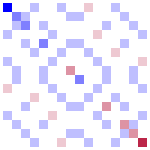
\includegraphics{imgs/3H.pdf}}\right), \hspace{5 mm} 
	\hat{U} = \left(\raisebox{-12mm}{
\includegraphics{imgs/3U.pdf}}\right), \hspace{5 mm} 
	\hat{U}\D\hat{H} \hat{U} = \left(\raisebox{-12mm}{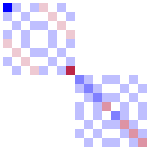
\includegraphics{imgs/3UHU.pdf}}\right). \hspace{5 mm} 
	\raisebox{-18mm}{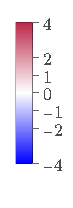
\includegraphics{imgs/3bl.pdf}}
\end{equation*}
where $\hat{U}$ represents reordering basis from
\begin{gather*}
	\ket{0000},\ket{0001},\ket{0010},\ket{0011},
	\ket{0100},\ket{0101},\ket{0110},\ket{0111}, \\
	\ket{1000},\ket{1001},\ket{1010},\ket{1011}, 
	\ket{1100},\ket{1101},\ket{1110},\ket{1111}
\end{gather*}
to 
\begin{gather*}
	\ket{0000},\ket{0011},\ket{0101},\ket{0110}, 
	\ket{1001},\ket{1010},\ket{1100},\ket{1111}, \\
	\ket{0001},\ket{0010},\ket{0100},\ket{0111},
	\ket{1000},\ket{1011},\ket{1101},\ket{1110}.
\end{gather*}


\begin{enumerate}[label=(\alph*)]
    \item To diagonalize $\hat{H}$ we could start from Fourier Transform
\begin{equation*}
	\hat{c}_k = \frac{1}{\sqrt{L}} \sum_j e^{i k j} \hat{c}_j,
	\hspace{10 mm} 
	\hat{c}_j = \frac{1}{\sqrt{L}} \sum_k e^{-i k j} \hat{c}_k.
\end{equation*}
Consider $L$ is even. If we want $\hat{c}_{L+1}= \hat{c}_1$ we have $H_1$ and
\begin{equation*}
	\mathcal K_{p=1} = \left\{
		k = \frac{\pi }{L}2n \ \big| \ n= - \tfrac{1}{2}L+1, \ldots, 0,\ldots,\tfrac{1}{2}L
	\right\},
\end{equation*}
otherwise $\hat{c}_{L+1} = - \hat{c}_1$ in $H_0$ and
\begin{equation*}
	\mathcal K_{p=0} = \left\{
		k =  \frac{ \pi }{L}(2n-1) \ \big| \  n= - \tfrac{1}{2}L+1, \ldots, 0,\ldots,\tfrac{1}{2}L
	\right\}.
\end{equation*}
And rewriting in terms of $\mathcal K_p$ hamiltonian we have
\begin{equation*}
	\hat{H}_{p} = -\sum_{k \in \mathcal K_p} (J \cos k + h) \left(
		\hat{c}\D_k \hat{c}_k - \hat{c}_{-k} \hat{c}\D_{-k}
	\right) - J \sum_{k \in \mathcal K_p} \left(e^{ik} \hat{c}_k\D \hat{c}_{-k}\D + \hc \right)
\end{equation*}

    \item It is useful to combine $k=0$ and $k=\pi$ for $p=1$
\begin{equation*}
	\hat{H}_{k=0,\pi} = - 2J (\hat{n}_0 - \hat{n}_\pi) + 2 h (\hat{n}_0 + \hat{n}_{\pi} - 2).
\end{equation*}
The remaining terms come into pairs $(k,-k)$, so we could go to the positive $k$:
\begin{align*}
	\mathcal K_1^+ &= \left\{
		k =  \frac{ \pi }{L}2n\ \big| \  n= 1,\ldots,\tfrac{1}{2}L-1
	\right\}, \\
	\mathcal K_0^+ &= \left\{
		k =  \frac{ \pi }{L}(2n-1) \ \big| \  n= 1,\ldots,\tfrac{1}{2}L
	\right\}.
\end{align*}
The $\hat{H}$ can be expressed as
\begin{equation*}
	\hat{H}_0 = \sum_{k \in \mathcal K_0^+} \hat{H}_k,
	\hspace{10 mm} 
	\hat{H}_1 = \hat{H}_{k=0,\pi} +  \sum_{k \in \mathcal K_1^+} \hat{H}_k,
\end{equation*}
with
\begin{equation*}
	\hat{H}_k = -2(J \cos k + h) \left(\hat{c}_k\D \hat{c}_k - \hat{c}_{-k} \hat{c}_{-k}\D\right) - 2 i J \sin k \left(
		\hat{c}_{k}\D \hat{c}_{-k}\D - \hat{c}_{-k} \hat{c}_{-k}
	\right).
\end{equation*}
Introducing $\hat{\Psi}\D_k = (\hat{c}_k\D,\ \hat{c}_{-k})$ we could simplify $\hat{H}_k$ to the
\begin{equation*}
	\hat{H} = \hat{\Psi}_k\D H_k \hat{\Psi}_k,
	\hspace{10 mm} 
	H_k = -2 J\begin{pmatrix}
	    -\tfrac{h}{J} + \cos k &  i \sin k \\
	    -  i \sin k & \tfrac{h}{J} - \cos k \\
	\end{pmatrix}.
\end{equation*}
Great, we have reduced the Hamiltonian to quadratic form and ready for the \textit{Bogolyubov transform}:
\begin{equation*}
	\hat{\Psi}_k = U \hat{\Phi}_k,
	\hspace{0.25cm} \Rightarrow \hspace{0.25cm}
	\hat{H}_k = \hat{\Phi}_k\D D_k \hat{\Phi}_k,
	\hspace{5 mm} 
	D_k = U\D H_k U = \begin{pmatrix}
	    \varepsilon_k & 0 \\
	    0 & -\varepsilon_k \\
	\end{pmatrix},
\end{equation*}
where $\hat{\Phi}_k\D \overset{\mathrm{def}}{=}   (\hat{\gamma}_k\D,\ \hat{\gamma}_{-k})$ -- our new operators. Diagonalizing $H_k$ we have
\begin{equation}
	U_k = \begin{pmatrix}
	    u_k & -\bar{v}_k \\
	    v_k & u_k \\
	\end{pmatrix} = 
	\frac{1}{\sqrt{\varepsilon_k(\varepsilon_k + z_k)}} \begin{pmatrix}
	    \varepsilon_k + z_k & i y_k \\
	    i y_k & \varepsilon_k + z_k \\
	\end{pmatrix},
	\hspace{5 mm} 
	\boxed{
	\varepsilon_k = 2 J \sqrt{\left(\cos k - \tfrac{h}{J}\right)^2 + \sin(k)^{2}}
	}
	\label{gap}
\end{equation}
where we introduced new parameters
\begin{equation*}
	u_k = \frac{\varepsilon_k + z_k}{\sqrt{\varepsilon_k (\varepsilon_k + z_k)}},
	\hspace{10 mm} 
	v_k = \frac{i y_k}{\sqrt{\varepsilon_k (\varepsilon_k + z_k)}},
	\hspace{10 mm} 
	\left.\begin{aligned}
    	z_k &= 2(h-J\cos k), \\
		y_k &= 2 J \sin k.
	\end{aligned}\right.
\end{equation*}
We could show that still
\begin{equation*}
	\{\hat{\gamma}_k, \hat{\gamma}_k\D\} = \{\bar{u}_k \hat{c}_k + \bar{v}_k \hat{c}\D_{-k},\ u_k \hat{c}_k\D + v_k \hat{c}_{-k}\} = |u_k|^2 + |v_k|^2 = 1,
\end{equation*}
so $\hat{\gamma}$ is a fermion. \red{Calculate commutators? But they are fermions!}


\end{enumerate}


	\item 
\begin{figure}[h]
    \centering
    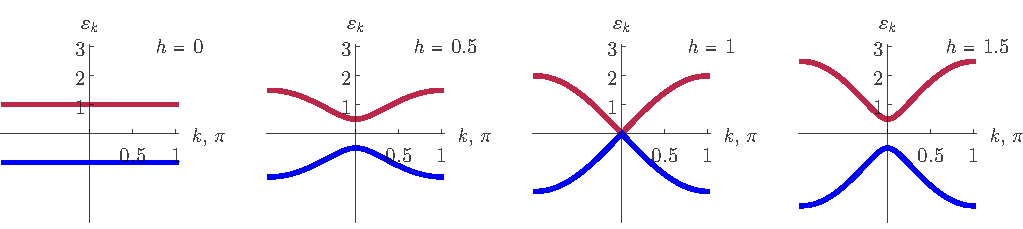
\includegraphics[width=0.9\textwidth]{imgs/3gap.pdf}
    \caption{TFIM dispersion with different magnetic fields $h$ with $J=1$}
    \label{fig:gap}
\end{figure}


\begin{enumerate}[label=(\alph*)]
    \item Ground state we could find in $\hat{H}_0$ such that $\hat{\gamma}_k \gs = 0 \ \forall k$. As in BCS theory we could start from some state (not orthogonal $\gs$), apply $\hat{\gamma}_k$ and normalize, coming to the
\begin{equation*}
	\gs = \frac{\prod_k \hat{\gamma}_{-k} \hat{\gamma}_k}{\left\|\prod_k \hat{\gamma}_{-k} \hat{\gamma}_k \ket{0}\right\|} \ket{0} = \prod_{k \in \mathcal K^+_0} \left(u_k + v_k \hat{c}_k\D \hat{c}\D_{-k}\right) \ket{0},
	\hspace{10 mm} 
	E_0 = - \sum_{k \in \mathcal K^+_0} \varepsilon_k,
\end{equation*}
with $\ket{0} \sim \ket{\downarrow\ldots\downarrow}$ -- vacuum for the original fermions $\hat{c}_k \ket{0} = 0 \ \forall k$. 
% \red{Add calculations of normalization.} 
% \red{Add proof that $p=1$ is not about ground state.} 
 If we want to continue exist in separated Hilbert space, than elementary excitation should save parity
\begin{equation*}
    \hat{\gamma}_{k_1}\D \hat{\gamma}_{k_2}\D \gs = \hat{c}_{k_1}\D \hat{c}_{k_2}\D \prod_{k \neq |k_1|,|k_2|}^{K^+_0} \left(\bar{u}_k - \bar{v}_k \hat{c}\D_k \hat{c}_{-k}\D \right) \ket{0}.
\end{equation*}
Going to the even amount of fermions we could apply even amount of $\hat{\gamma}_k$ to the $\gs$.
    \item Gap between minimal exitation and $\gs$ is $\varepsilon_{k=0}$,
% (we go from $-\varepsilon_k$ to the $\varepsilon_k$, that how 2-factor appear)
 and gap in $\varepsilon_k$ disappear at $h/J=1$ (fig. \ref{fig:gap}). Interesting to plot all $\hat{H}$ eigenvalues and see what is happening in the same values of $h$ (fig. \ref{fig:F}). 




\begin{figure}[h]
    \centering
    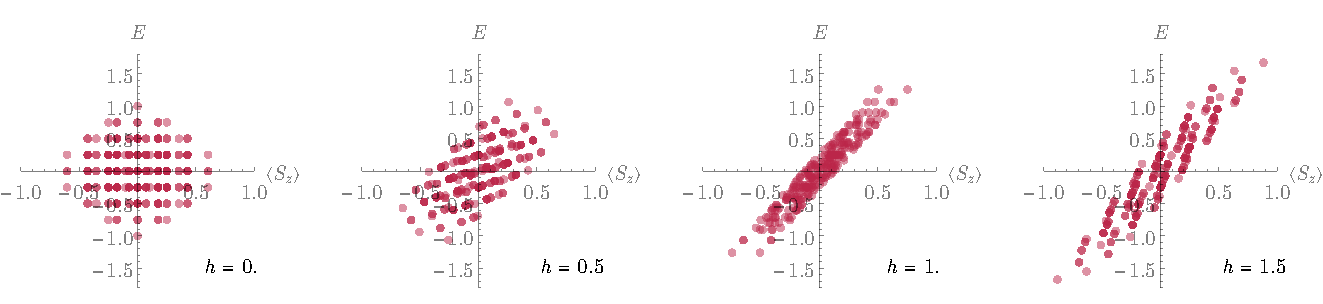
\includegraphics[width=0.9\textwidth]{imgs/3F.pdf}
    \caption{Eigenvalues of $\hat{H}$ as a function of $\langle S_z\rangle$}
    \label{fig:F}
\end{figure}

\end{enumerate}
 \newpage
	\item Consider $\xi$ as
\begin{equation*}
	f(r) = \left\langle \sigma_j^z \sigma_{j+r}\right\rangle \propto e^{- r /\xi},
\end{equation*}
so we could estimate it numerically (fig. \ref{fig:raf}). We have finite $L$ that strongly affects $\xi$ estimation, but definitely something interesting happens at $h=\sub{h}{c}=1$.

 We know that
\begin{equation*}
	\frac{1}{\sub{E}{gap} }  \propto \frac{1}{\varepsilon_{k=0}} \propto  \xi^{z} \propto (h - \sub{h}{c})^{-\nu z},
\end{equation*}
and from \eqref{gap} at $k=0$ we have $\sub{E}{gap} \propto h-1$, than $\sub{h}{c}=1$ and $\nu z = 1$.

\begin{figure}[h]
    \centering
    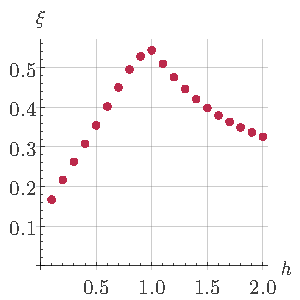
\includegraphics[width=0.25\textwidth]{imgs/3rad.pdf}
    \caption{Correlation radius $\xi$ as a function of external magnetic field $h$ at $L=20$, ground state}
    \label{fig:raf}
\end{figure}

\end{enumerate}


% 
\phantom{42}

\vfill

\phantom{42} \hfill \textbf{\textit{\today, \ Khoruzhii Kirill}}


% \newpage
% \setcounter{section}{4}
% \setcounter{subsection}{0}
% \subsection{Feynman Path Integral of the Harmonic Oscillator}
% Consider propagator as 
\begin{equation*}
	K \overset{\mathrm{def}}{=}  \bk{q_f}[e^{-i \hat{H} T}]{q_i},
\end{equation*}
that we could rewrite in terms of the Feinman's integral
\begin{equation*}
	K = \int e^{i S[q(t)]} \F q(t),
\end{equation*}
with in particular action for the harmonic oscillator
\begin{equation}
	S[q(t)] = \int_{0}^{T} \frac{m}{2} \left(
		\dot{q}^2 - \omega^2 q^2
	\right)
	\label{S}
\end{equation}
with boundary conditions $q(0) = q_i$ and $q(T) = q_f$. 

\begin{enumerate}[label=(\alph*)]
    
    \item Writing the path as $q(t) = q_c(t) = y(t)$, due to $\delta S[q_c(t)] = 0$ we could rewrite $S$ as 
\begin{equation*}
	S[q(t)] = \int_{0}^{T} \frac{m}{2}\left(
		(\dot{q}_c + \dot{y})^2 - \omega^2 (q_c + y)^2
	\right) \d t = S[q_c(t)] + S[y(t)] + \int_{0}^{T} m\left(
		\dot{q}_c \d y - \omega^2 q_c y \d t
	\right)  = S[q_c(t)] + S[y(t)].
\end{equation*}
It was used that Euler-Lagrange equation $\partial_x L - \frac{d }{d t} \partial_{\dot{x}} L = 0$ leads to classical equation of motion $\ddot{q}_c = - m \omega^2 q_c(t)$:
\begin{equation*}
	\int_{0}^{T}  m \dot{q}_c \d y = y(t) \dot{q}_c \bigg|_0^T - \int_{0}^{T} m y \ddot{q}_c \d t = \int_{0}^{T}  m \omega^2 y q_c \d t. 
\end{equation*}
Thus we could factorise $K$
\begin{equation*}
	K = e^{i S[q_c(t)]} F(T),
	\hspace{10 mm} 
	F(T) = \int e^{i S[y(t)]} \F y(t).
\end{equation*}

    \item Solving $\ddot{q}_c = - m \omega^2 q_c(t)$ with boundary conditions $q(0) = q_i$ and $q(T) = q_f$ we get
\begin{equation*}
	q_c(t) = A \cos (\omega t) + B \sin (t),
	\hspace{0.25cm} \Rightarrow \hspace{0.25cm}
	\left\{\begin{aligned}
	    q_i &= B \\
	    q_f &= A \sin(\omega T) + B \cos(\omega T)
	\end{aligned}\right.
	\hspace{0.25cm} \Rightarrow \hspace{0.25cm}
	A = \frac{q_f - q_i \cos(\omega T)}{\sin(\omega T)},
	\hspace{2.5 mm} 
	B = q_i,
\end{equation*}
and substituting into the action \eqref{S}
\begin{equation*}
	S[q_c(t)] = \frac{m \omega}{2 \sin(\omega T)} \left(
		(q_i^2 +q_f^2) \cos(\omega T) - 2 q_i q_f
	\right).
\end{equation*}
    \item The fluctuations can be expressed as a Fourier series
\begin{equation*}
	y(t) = \sum_{n=1}^{\infty} a_n \sin\left(
		\frac{n \pi t}{T}
	\right),
\end{equation*}
we go to the integration over $\prod_n a_n$. It is useful to calculate
\begin{equation*}
	\int_{0}^{T} \dot{y}^2 \d t = \frac{T}{2} \sum_{n=1}^{\infty} \left(\frac{\pi n}{T}\right)^2 a_n^2,
	\hspace{10 mm} 
	\int_{0}^{T} y^2 \d t = \frac{T}{2} \sum_{n=1}^{\infty} a_n^2.
\end{equation*}
So we could find $F$ as
\begin{equation*}
	F(T) \propto \int \exp\left(
		-\sum_{n=1}^{\infty} \alpha_n  a_n^2
	\right) \prod_n \d a_n = \prod_{n=1}^{\infty} \sqrt{\frac{\pi}{\alpha_n}},
	\hspace{10 mm} 
	\alpha_n = \frac{m}{2 i \hbar}\frac{T}{2} \left(\frac{\pi n}{T}\right)^2 \left(1 - \frac{\omega^2 T^2}{n^2 \pi^2}\right) .
\end{equation*}
Ignoring all factors without $\omega$, we have
\begin{equation*}
	F(T) = C \prod_{n=1}^{\infty} \left(1 -  \frac{\omega^2 T^2}{n^2 \pi^2}\right)^{-1/2} = C \sqrt{\frac{\omega T}{\sin (\omega T)}},
\end{equation*}
with some constant $C$ that could be find from the free particle case $\omega \to 0$
\begin{equation*}
	\lim_{\omega \to 0} F(T) = C = \sqrt{\frac{m}{2\pi i \hbar T}},
	\hspace{0.5cm} \Rightarrow \hspace{0.5cm}	
	F(T) = \sqrt{\frac{m \omega}{2\pi i \hbar \sin(\omega T)}}.
\end{equation*}
    \item[(d, e)] Now we could calculate the partition function $Z = \tr e^{- \beta \hat{H}}$ after a Wick rotation to imaginary times $T = - i \beta$
\begin{equation*}
	Z = \int \bk{x}[e^{- \beta \hat{H}}]{x} \d x = \int e^{i S[q_c(-i \beta)]}F(-i \beta) \d x \overset{(1)}{=}  \frac{1}{2 \sh\left(\tfrac{1}{2} \omega \beta\right)},
\end{equation*}
where in $\overset{(1)}{=}$ we calculated Gaussian integral 
\begin{equation*}
	\int \exp(- \alpha x^2) \d x = \sqrt{\frac{\pi}{\alpha}},
	\hspace{10 mm} 
	\alpha = \frac{ i m \omega \left(1 - \cos (\omega T)\right)}{\sin (\omega T)}.
\end{equation*}

\end{enumerate}





% \subsection{Grassmannian Algebra (I)}

We know, that for the Grassmann number $\eta$
\begin{equation*}
	\int \eta \d \eta = 1,
	\hspace{10 mm} 
	\int \d \eta = 0.
\end{equation*}

\begin{enumerate}
	\item Interesting to note, that for $f(\eta) = a + b \eta$ ($a,\, b \in \mathbb{C}$) we have
\begin{equation*}
	\{\eta,\, \partial_\eta\} f(\eta) = \{\eta,\, \textstyle \int d \eta\} f(\eta) = f(\eta).
\end{equation*}
Enough to calculate
\begin{equation*}
\textstyle
	\eta \int d \eta f(\eta) = b \eta,
	\hspace{5 mm} 
	\eta \partial_\eta f(\eta) = b \eta,
	\hspace{5 mm} 
	\int d \eta \eta  f(\eta) = a,
	\hspace{5 mm} 
	\partial_\eta \eta  f(\eta) = a.
\end{equation*}
	\item As a next step we calculate 
\begin{equation*}
	\exp\left(
		\sum_j c_j \eta_j
	\right) = 1 + \sum_j c_j \eta_j + 
	\sum_{j,k} c_j c_k \eta_j \eta_k = 
	 1 + \sum_j c_j \eta_j + 
	\sum_{j>k} c_j c_k (\eta_j \eta_k+\eta_k \eta_j) =  1 + \sum_j c_j \eta_j 
	,
\end{equation*}
with $c_j \in \mathbb{C}$. Actually it is the same as proof that $\sum_j c_j \eta_j $ is still Grassmann number by calculating anticommutative relations.
	\item Finally, we could find integral
\begin{equation*}
	\int d \bar{\eta} d \eta \ e^{- C \bar{\eta} \eta} = 
	\int d \bar{\eta} d \eta \left(
		1 - C \bar{\eta} \eta + \tfrac{C^2}{2} \bar{\eta}  \eta \bar{\eta} \eta + \ldots
	\right) = C \int d \bar{\eta} \left(
		\int d \eta\ \eta \bar{\eta}
	\right) = C,
\end{equation*}
with $C \in \mathbb{C}$. It was used that $\bar{\eta}  \eta \bar{\eta} \eta = - \bar{\eta}^2 \eta^2 = 0$.
\end{enumerate}


% \newpage
\setcounter{section}{5}
\setcounter{subsection}{0}
\subsection{Complex analysis}
Consider Gaussian integral 
\begin{equation*}
	I_1 = \int_{-\infty}^{\infty} e^{-i a x^2} \d x,
\end{equation*}
with $\alpha \in \mathbb{R}^+$. We could use that
\begin{equation*}
	I_2 = \int_{-\infty}^{\infty} e^{-b x^2} \d x = \sqrt{\frac{\pi}{a}}.
\end{equation*}
Define  $\mathcal C_1 = \{z=e^{i \frac{\pi}{4}x} \colon x \in \mathbb{R}\}$,
$\mathcal C_2 = \{z=x \colon x \in \mathbb{R}\}$ and ${\mathcal C}_R^\pm = \{z = \pm R e^{i \varphi} \colon \varphi \in [0, \pi/4]\}$. Applying Cauchy integral theorem for holomorphic functions to the $\mathcal C = \mathcal C_1 \cup \mathcal C_2 \cup {\mathcal C}_R^+ \cup {\mathcal C}_R^-$ we have 
\begin{equation*}
	-I[\mathcal C_1]+I[\mathcal C_2]+I[{\mathcal C}_R^+]+I[{\mathcal C}_R^-] = 0,
\end{equation*}
with $I[\mathcal C_1] e^{-i \frac{\pi}{4}} = I_1 $, $I[\mathcal C_2] = I_2$.

The $I[{\mathcal C}_R^\pm]$ could be estimated as
\begin{equation*}
	|I[{\mathcal C}_{R \to \infty}^\pm] | \leq \lim_{R \to \infty} \int_{0}^{\pi/2} e^{-a R^2 \varphi} r \d \varphi = \lim_{R \to \infty} \frac{1}{aR}\left(
		1 - e^{- \frac{1}{2} a \pi r^2}
	\right) = 0,
\end{equation*}
thus we have
\begin{equation*}
	I_1 = I[\mathcal C_1] e^{-i \frac{\pi}{4}} =  I[\mathcal C_2] e^{-i \frac{\pi}{4}} = e^{-i \frac{\pi}{4}} \sqrt{\frac{\pi}{a}},
\end{equation*}
that could be generalized as
\begin{equation*}
	\int_{-\infty}^{\infty} e^{\pm i a x^2} \d x = e^{\pm i \frac{\pi}{4}} \sqrt{\frac{\pi}{a}}.
\end{equation*}



\subsection{Effective action of coupled harmonic oscillators}
We could derive the low-energy effective action for a system of two
coupled harmonic oscillators, formally described by the classical partition function
\begin{equation*}
	Z = \int Dx DX \, \exp\left(
		i \int dt\ L(x, X, \dot{x}, \dot{X}) 
	\right),
\end{equation*}
with
\begin{equation*}
	L = \frac{1}{2} m \dot{x}^2 - \frac{1}{2} m \omega^2 x^2 + \frac{1}{2} M \dot{X}^2 - \frac{1}{2} M \Omega^2 X^2 - g X x.
\end{equation*}
It could be expanded as
\begin{equation*}
	Z = \int Dx \ e^{i S_0 + i\sub{S}{int}},
	\hspace{5 mm} 
	e^{ i\sub{S}{int}} = \int D X \ \exp\left(
		i \int \d t \left[
			\tfrac{1}{2} M \dot{X}^2 - \tfrac{1}{2} M \Omega^2 X^2 - g X x
		\right]
	\right).
\end{equation*}
Integrating by parts we have Gaussian integral that coul be calculated directly
\begin{equation*}
	e^{ i\sub{S}{int}} = \int D X \ \exp\left(
		i \int \d t \left[
			\tfrac{1}{2} M X(\partial_t^2+ \Omega^2)X - g X x
		\right]
	\right) = \mathcal N \exp\left(
		i \int dt \frac{g^2}{2M} x \left(\partial_t^2 + \Omega^2\right)^{-1} x
	\right)
\end{equation*}
with $\mathcal N$ as some irrelevant normalizing factor. That leads to some $\sub{L}{eff}$
\begin{equation*}
	\sub{L}{eff} = \tfrac{1}{2} m \ddot{x}^2 - \frac{1}{2} m x^2 \sub{\omega}{eff}^2,
	\hspace{10 mm} 
	\sub{\omega}{eff} =  \omega \sqrt{1 - \alpha^2 \frac{m}{M} \left(\frac{\omega}{\Omega}\right)^2},
\end{equation*}
with $g = \alpha m \omega^2$ and, apparently, $\sub{m}{eff} = m$.






% 
\phantom{42}

\vfill

\phantom{42} \hfill \textbf{\textit{\today, \ Khoruzhii Kirill}}


% 18, 
% 14, Ahmed Omran’s PhD thesis
% Dominant Fifth-Order Correlations in Doped Quantum Antiferromagnets
% Omran, A. A microscope for Fermi gases. (2016).

% SW: you can use this figure to help explain string model if you want
% Parton Theory of Magnetic Polarons: Mesonic Resonances and Signatures in Dynamics

% Coupling a Mobile Hole to an Antiferromagnetic Spin Background: Transient Dynamics of a Magnetic Polaron


% \begin{itemize}
% 	\item ${}^{6}$Li
% 	\item $t_y / h \approx t_x / h = 170\,$Hz
% 	\item $U / t = 14(1)$
% 	\item $J / h = 50(5)\,$Hz
% 	\item $T \approx 1.4 J$
% \end{itemize}

% Grusdt at all. ‘Parton Theory of Magnetic Polarons: Mesonic Resonances and Signatures in Dynamics’. Physical Review X 8, no. 1 (21 March 2018): 011046. https://doi.org/10.1103/PhysRevX.8.011046.


% 20 слайд
